% !Mode:: "TeX:UTF-8" 



\BiSection{2.12}{Figures}

\fancyhead[R]{本题2.12由QC.Z完成}

对于图2.54的每个电路,画出$V_X$关于时间的函数曲线草图,每个电容器的初始电压如图所示。

		\begin{figure}[H] %H为当前位置,!htb为忽略美学标准,htbp为浮动图形
	\begin{minipage}{\linewidth}
		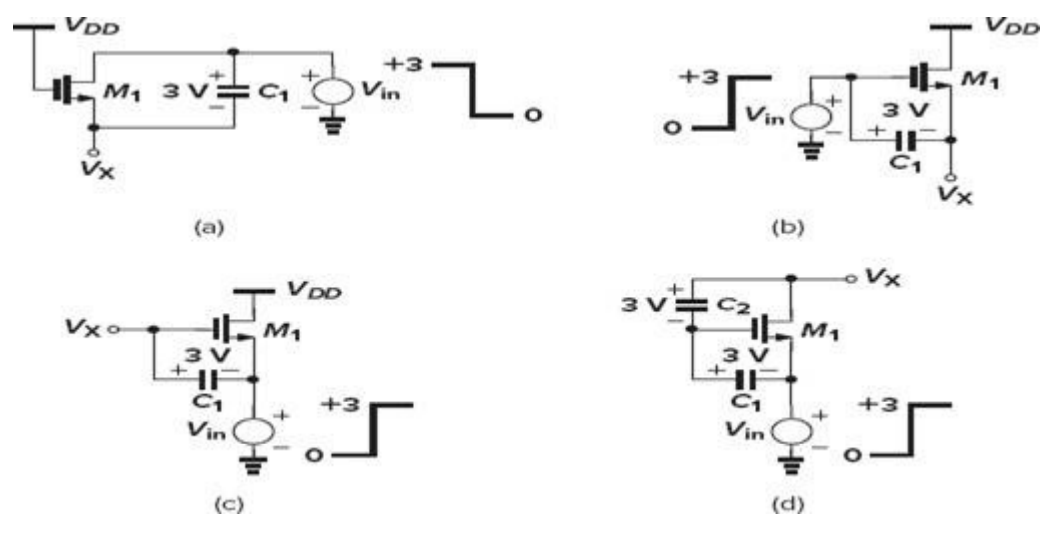
\includegraphics[width=1\linewidth]{2.12.54}
	\end{minipage}
	\caption*{图2.54} %最终文档中希望显示的图片标题
\end{figure}

解:

\scalebox{3}{(a)}

当$V_{in}$为3V时,因为$C_1$电压为3V,所以$V_X$为0V;当$V_{in}$为0V时,因为$C_1$电压为3V,所以$V_X$为-3V

(a)重画于图1

		\begin{figure}[H] %H为当前位置,!htb为忽略美学标准,htbp为浮动图形
	\begin{minipage}{\linewidth}
		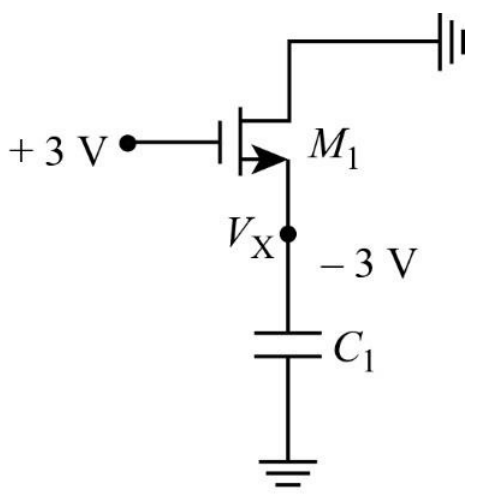
\includegraphics[width=1\linewidth]{2.12-1}
	\end{minipage}
	\caption*{图1} %最终文档中希望显示的图片标题
\end{figure}

$V_X$端电压低为源,接地端电压高为漏。当$t \geqslant 0^+$时,$V_{GS}-V_{TH}>V_{DS}$即3V-0.7V>0V,NFET在线性区

$I_D=\frac{1}{2}\mu_nC_{ox}\frac{W}{L}[2(V_{GS}-V_{TH})V_{DS}-V_{DS}^2]=\frac{1}{2}\mu_nC_{ox}\frac{W}{L}[2(2.3-V_X)(-V_{X})-V_{X}^2]$

$I_D=C_1\frac{dV_X}{dt}$

联立以上二式

\begin{figure}[H] %H为当前位置,!htb为忽略美学标准,htbp为浮动图形
	\begin{minipage}{\linewidth}
		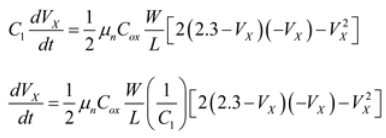
\includegraphics{2.12-2}
	\end{minipage}
\end{figure}

令$\alpha=(\frac{1}{2}\mu_nC_{ox}\frac{W}{L})(\frac{1}{C_1})$

\begin{figure}[H] %H为当前位置,!htb为忽略美学标准,htbp为浮动图形
	\begin{minipage}{\linewidth}
		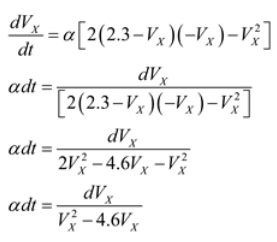
\includegraphics{2.12-3}
	\end{minipage}
\end{figure}

\begin{figure}[H] %H为当前位置,!htb为忽略美学标准,htbp为浮动图形
	\begin{minipage}{\linewidth}
		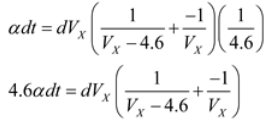
\includegraphics{2.12-4}
	\end{minipage}
\end{figure}

\begin{figure}[H] %H为当前位置,!htb为忽略美学标准,htbp为浮动图形
	\begin{minipage}{\linewidth}
		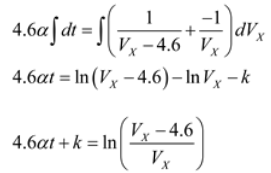
\includegraphics{2.12-5}
	\end{minipage}
\end{figure}

\begin{figure}[H] %H为当前位置,!htb为忽略美学标准,htbp为浮动图形
	\begin{minipage}{\linewidth}
		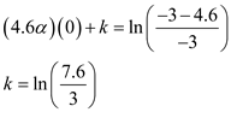
\includegraphics{2.12-6}
	\end{minipage}
\end{figure}

\begin{figure}[H] %H为当前位置,!htb为忽略美学标准,htbp为浮动图形
	\begin{minipage}{\linewidth}
		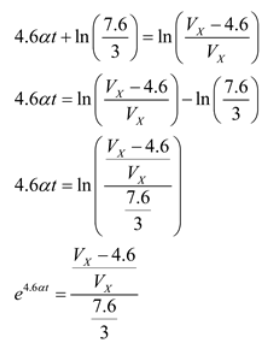
\includegraphics{2.12-7}
	\end{minipage}
\end{figure}

\begin{figure}[H] %H为当前位置,!htb为忽略美学标准,htbp为浮动图形
	\begin{minipage}{\linewidth}
		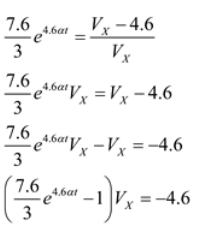
\includegraphics{2.12-8}
	\end{minipage}
\end{figure}


$V_X=\frac{-4.6}{\frac{7.6}{3}e^{4.6 \alpha t}-1}$

\begin{figure}[H] %H为当前位置,!htb为忽略美学标准,htbp为浮动图形
	\begin{minipage}{\linewidth}
		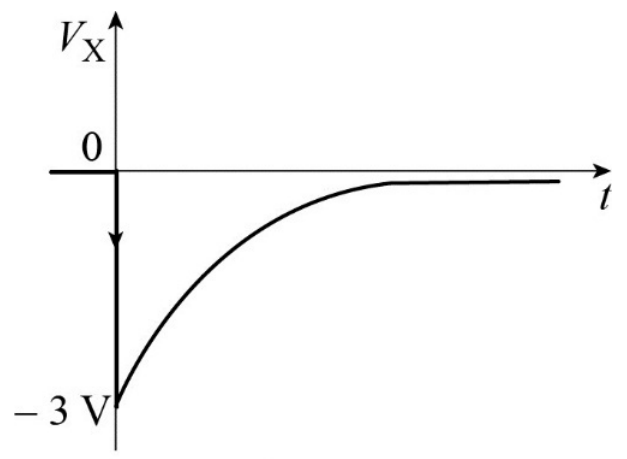
\includegraphics[width=1\linewidth]{2.12-9}
	\end{minipage}
	\caption*{图2} %最终文档中希望显示的图片标题
\end{figure}

\color{blue}{
	
	\{
	
	$t=0^+$时电容的电流不会直接流入地吗?反证法,$t=0^+$时假设电容正极板从地接收电子,这样负极板等量电子会被正极板排斥到地,结论是电容的电流不会流入地。
	
	假设$V_{in}$从3变0时$t=t_0$,如果$t_0$是器件截止时刻则$V_X$在此时从2.3跳到-0.7;如果$t_0$在器件截止之前,并且此时$V_X$电压为$\epsilon$,这样时间刚越过$t_0$时,$V_X$电压为$\epsilon$-3。如果在理想情况时$t_0$足够小,就是正文中的情况。
	
	\}
	
}
\color{black}{}

\scalebox{3}{(b)}

当$V_{in}$为0V时,因为$C_1$电压为3V,所以$V_X$为-3V;当$V_{in}$为3V时,因为$C_1$电压为3V,所以$V_X$为0V

(b)重画于图3

		\begin{figure}[H] %H为当前位置,!htb为忽略美学标准,htbp为浮动图形
	\begin{minipage}{\linewidth}
		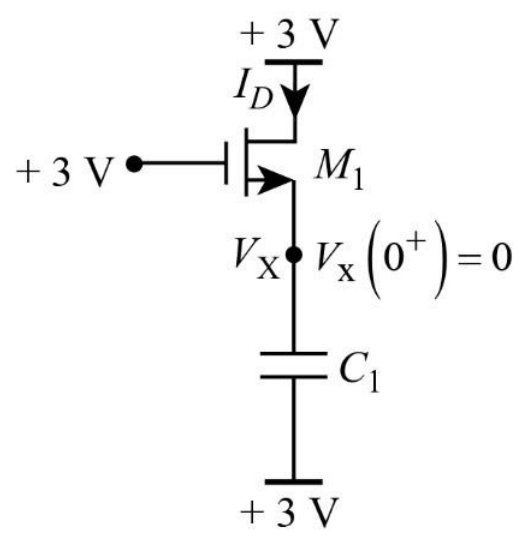
\includegraphics[width=1\linewidth]{2.12-10}
	\end{minipage}
	\caption*{图3} %最终文档中希望显示的图片标题
\end{figure}

$V_{D}>V_{G}-V_{TH}$即$3V>2.3V$($t \geqslant 0^+$),饱和区$I_D=\frac{1}{2}\mu_nC_{ox}\frac{W}{L}(3V-V_X-0.7V)^2$

$I_D=C_1\frac{dV_X}{dt}$

联立以上二式

$\frac{1}{2}\mu_nC_{ox}\frac{W}{L}(2.3V-V_X)^2(\frac{1}{C_1})=\frac{dV_X}{dt}$

令$\alpha=(\frac{1}{2}\mu_nC_{ox}\frac{W}{L})(\frac{1}{C_1})$

$\alpha (2.3V-V_X)^2=\frac{dV_X}{dt}$

$\alpha \int dt =\int \frac{dV_X}{(2.3V-V_X)^2}$

$\alpha t+k=\frac{1}{2.3V-V_X}$\ding{172}

$(\alpha) (0)+k=\frac{1}{2.3V-0V}$

$k=\frac{1}{2.3V}$

将上式代入\ding{172}

$\alpha t+\frac{1}{2.3V}=\frac{1}{2.3V-V_X}$

\begin{figure}[H] %H为当前位置,!htb为忽略美学标准,htbp为浮动图形
	\begin{minipage}{\linewidth}
		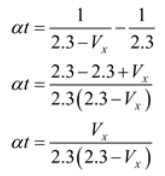
\includegraphics{2.12-11}
	\end{minipage}
\end{figure}

\begin{figure}[H] %H为当前位置,!htb为忽略美学标准,htbp为浮动图形
	\begin{minipage}{\linewidth}
		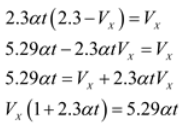
\includegraphics{2.12-12}
	\end{minipage}
\end{figure}

\begin{figure}[H] %H为当前位置,!htb为忽略美学标准,htbp为浮动图形
	\begin{minipage}{\linewidth}
		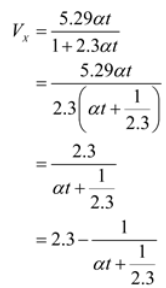
\includegraphics{2.12-13}
	\end{minipage}
\end{figure}

		\begin{figure}[H] %H为当前位置,!htb为忽略美学标准,htbp为浮动图形
	\begin{minipage}{\linewidth}
		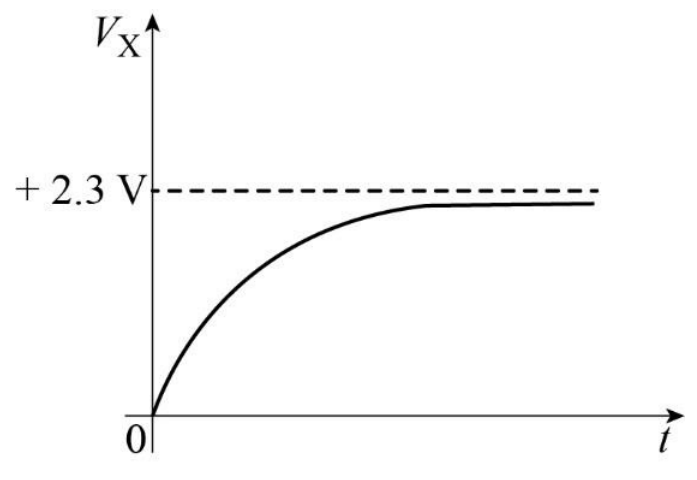
\includegraphics[width=1\linewidth]{2.12-14}
	\end{minipage}
	\caption*{图4} %最终文档中希望显示的图片标题
\end{figure}

\scalebox{3}{(c)}

$V_G-V_{TH}>V_{D}$即$3V+3V-0.7V>3V$,用线性区公式$I_D=\frac{1}{2}\mu_nC_{ox}\frac{W}{L}[2(V_{GS}-V_{TH})V_{DS}-V_{DS}^2]=\frac{1}{2}\mu_nC_{ox}\frac{W}{L}[2(V_{GS}-V_{TH})(3V-3V)-(3V-3V)^2]=0$

		\begin{figure}[H] %H为当前位置,!htb为忽略美学标准,htbp为浮动图形
	\begin{minipage}{\linewidth}
		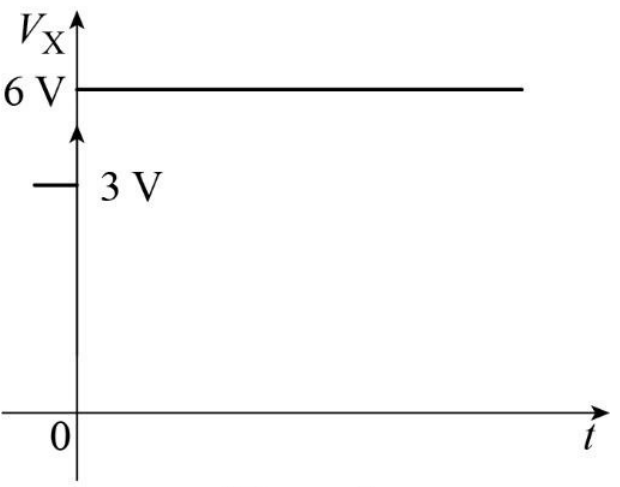
\includegraphics[width=1\linewidth]{2.12-15}
	\end{minipage}
	\caption*{图5} %最终文档中希望显示的图片标题
\end{figure}

\scalebox{3}{(d)}

因为$t=0^+$两电容器负极板电子同时流向对方正极板,由电荷守恒定律,两电容器通过源漏的电流等于栅这边两电容器电流并且$V_X$只有两端;所以$V_{in}$没有电流

$t=0^+$时$V_G=V_{in}+V_{C1}=6V$且$V_D=V_{in}+V_{C1}+V_{C2}=9V$,$V_G-V_{TH}<V_{D}$即$6V-0.7V<9V$NFET在饱和区

\scalebox{2}{(1)}

情况一:$C_2$电压减得很快且变为某一负值,$V_G-V_{TH}=V_{in}+V_{C1}-V_{TH}>V_D=V_{in}+V_{C1}+V_{C2}$即$V_{C2}<-0.7V$时NFET进入线性区,过程中$V_X=V_D$因$V_{C2}$项减小。直到$V_G$>$V_D=V_{in}=3V$,此时$V_{DS}=0,I_D=0$NFET关,$V_X=V_D=V_S=3V$\textcolor{blue}{($C=\frac{Q}{U}$即此情况下$C_2$小或$C_1$大)}

此情况下先在饱和区电流下降慢同时$V_X$因为$C_2$而下降较快,后在线性区电流下降快同时$V_X$因为$C_2$而下降较慢,最终$V_X=V_D=V_S=3V$。也可用饱和区和线性区电流公式做与其他题目类似的分析。图略。

\scalebox{2}{(2)}

情况二:$C_1$电压减得很快,$V_{GS}=V_{C1}$很快等于阈值电压,NFET关,$V_X=V_{in}+V_{C1}+V_{C2}$\textcolor{blue}{(过程中一直在饱和区,因为$V_{in}+V_{C1}-V_{TH}<V_{in}+V_{C1}+V_{C2}$即$V_G-V_{TH}<V_{D}$)}








$V_{GS}=V_{C1}=3-\frac{1}{C_1} \int I_Ddt=3-\frac{q}{C_1}$

$V_{DG}=V_{C2}=3-\frac{1}{C_2} \int I_Ddt=3-\frac{q}{C_2}$

%$C_1<1.61C_2$










%$V_{D}>V_{G}-V_{TH}$即$3V>2.3V$($t>0$),饱和区$I_D=\frac{1}{2}\mu_nC_{ox}\frac{W}{L}(3V-\frac{q}{C_1}-0.7V)^2$

饱和区$I_D=\frac{1}{2}\mu_nC_{ox}\frac{W}{L}(3V-\frac{q}{C_1}-0.7V)^2$




$\frac{dq}{dt}=\frac{1}{2}\mu_nC_{ox}\frac{W}{L}(3V-\frac{q}{C_1}-0.7V)^2$

$\frac{\frac{dq}{C_1}}{dt}=\frac{1}{2}\mu_nC_{ox}\frac{W}{L}(\frac{1}{C_1})(3V-\frac{q}{C_1}-0.7V)^2$

令$\alpha=(\frac{1}{2}\mu_nC_{ox}\frac{W}{L})(\frac{1}{C_1})$

\begin{figure}[H] %H为当前位置,!htb为忽略美学标准,htbp为浮动图形
	\begin{minipage}{\linewidth}
		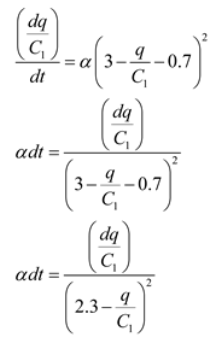
\includegraphics{2.12-16}
	\end{minipage}
\end{figure}

\begin{figure}[H] %H为当前位置,!htb为忽略美学标准,htbp为浮动图形
	\begin{minipage}{\linewidth}
		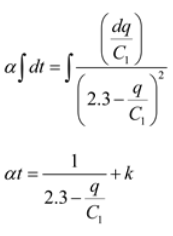
\includegraphics{2.12-17}
	\end{minipage}
\end{figure}

\begin{figure}[H] %H为当前位置,!htb为忽略美学标准,htbp为浮动图形
	\begin{minipage}{\linewidth}
		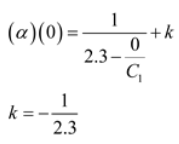
\includegraphics{2.12-18}
	\end{minipage}
\end{figure}

\begin{figure}[H] %H为当前位置,!htb为忽略美学标准,htbp为浮动图形
	\begin{minipage}{\linewidth}
		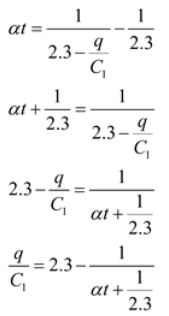
\includegraphics{2.12-19}
	\end{minipage}
\end{figure}

\begin{figure}[H] %H为当前位置,!htb为忽略美学标准,htbp为浮动图形
	\begin{minipage}{\linewidth}
		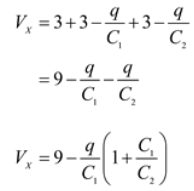
\includegraphics{2.12-20}
	\end{minipage}
\end{figure}

\begin{figure}[H] %H为当前位置,!htb为忽略美学标准,htbp为浮动图形
	\begin{minipage}{\linewidth}
		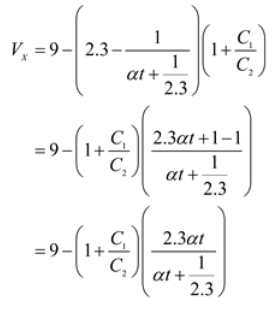
\includegraphics{2.12-21}
	\end{minipage}
\end{figure}

\begin{figure}[H] %H为当前位置,!htb为忽略美学标准,htbp为浮动图形
	\begin{minipage}{\linewidth}
		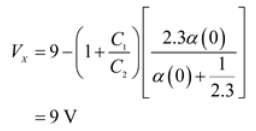
\includegraphics{2.12-22}
	\end{minipage}
\end{figure}


		\begin{figure}[H] %H为当前位置,!htb为忽略美学标准,htbp为浮动图形
	\begin{minipage}{\linewidth}
		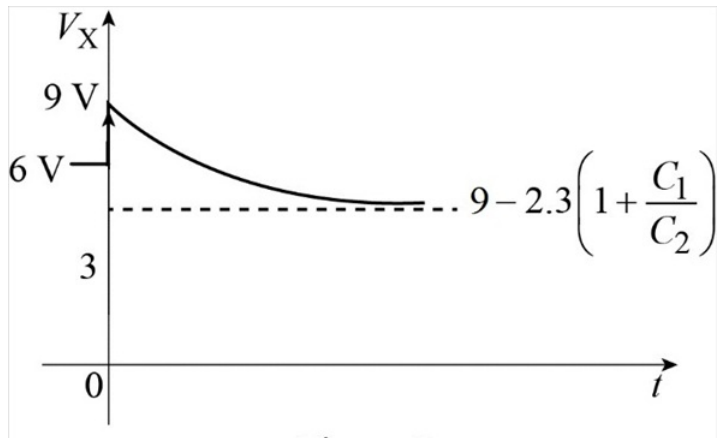
\includegraphics[width=1\linewidth]{2.12-23}
	\end{minipage}
	\caption*{图6} %最终文档中希望显示的图片标题
\end{figure}

\color{green}{

\{

(d)未完善有待补充


\}

}
\color{black}{}